% Section 1.4: Indirect Detection via Gamma-Rays (The Formalism)
% Structure: Annihilation/decay physics -> Spectral signatures -> Density profiles -> J/D-factor -> Targets -> Multi-messenger -> Status

\section{Indirect Detection via Gamma-Rays}
\label{sec:1.4}

\blue{In our efforts to better understand the potential particle nature of dark matter, we now steer our attention towards indirect detection searches.}
Indirect detection via gamma-rays directly probes the annihilation cross-section --- the quantity that governs the thermal relic abundance and the one quantity that underground laboratories cannot access.
This section derives the relevant equations for the gamma-rays flux, which is key to every analysis presented in this thesis.
% This section develops the underlying formalism.
% We follow the signal from particle physics --- the annihilation and decay rates, the spectra they produce --- through astrophysics --- the density profiles that determine where the dark matter sits --- to derive the equations that predict the gamma-ray flux from any given target.
% These expressions, and the assumptions that enter them, provide the quantitative foundation for every analysis presented in this thesis.

\blue{We first consider the microphysics of annihilation and decay and the gamma-ray spectra they produce (\S\ref{sec:ann_decay}--\S\ref{sec:spectral_features}), then introduce the dark matter density profiles that determine how the signal varies across the sky (\S\ref{sec:density_profiles}).
These ingredients combine into the $J$-factor and $D$-factor formalism, which factorizes the predicted flux into a particle-physics term and an astrophysical term (\S\ref{sec:jfactor}). We then survey the observational targets that define the thesis programme (\S\ref{sec:targets}--\S\ref{sec:status}).}

\subsection{Annihilation and Decay Physics}
\label{sec:ann_decay}

In the $\Lambda$CDM framework, structure forms hierarchically from cold, non-relativistic dark matter, and the particles that populate present-day galactic halos retain typical velocities of order $v \sim 10^{-3}\, c$ \cite{Hooper:2024}.
They therefore annihilate or decay essentially at rest.
This kinematic fact has two immediate consequences.
First, the total center-of-mass energy available in an annihilation event \blue{today is roughly} $\sqrt{s} = 2 m_\chi$, so the most energetic photon that can be produced carries energy $E_\gamma = m_\chi$.
For decay, the available energy is instead $m_\chi$, and momentum conservation among at least two daughter particles limits the maximum photon energy to $E_\gamma = m_\chi / 2$.
These hard kinematic endpoints are among the most distinctive features of a dark matter signal, since known astrophysical gamma-ray sources do not generically produce spectra with such a sharp cutoff tied to a single mass scale.

The second consequence is more profound and concerns the spatial morphology of the expected signal.
Annihilation is a two-body process and its rate per unit volume is therefore proportional to the square of the local dark matter density:
%
\begin{equation}
	\frac{d\Gamma_\text{ann}}{dV} = \frac{\langle \sigma v_\text{rel} \rangle}{2} \frac{\rho^2}{m_\chi^2} \,,
	\label{eq:ann_rate}
\end{equation}
%
where $\langle \sigma v_\text{rel} \rangle$ is the thermally averaged annihilation cross-section and the factor of $1/2$ avoids double-counting for self-conjugate particles \cite{Hooper:2024}.
For Dirac dark matter, where particle and antiparticle are distinct, the factor becomes $1/4$, but the thermal cross-section required for the correct relic abundance is correspondingly larger, leaving the observable rate unchanged \cite{Hooper:2024}.
Decay, by contrast, is a single-particle process with a rate proportional to the first power of the density:
%
\begin{equation}
	\frac{d\Gamma_\text{dec}}{dV} = \frac{\rho}{m_\chi \tau} \,,
	\label{eq:dec_rate}
\end{equation}
%
where $\tau$ is the dark matter lifetime \cite{Hooper:2024}.
% Current gamma-ray observations constrain $\tau \gtrsim 10^{28}$ s \cite{Cohen:2016uyg,Blanco_2019}, far exceeding the age of the universe --- making decay an intrinsically rare process whose detection requires enormous integrated exposures.
\blue{Current gamma-ray constraints place $\tau$ some ten orders of magnitude beyond the age of the universe (the numbers are collected in Section~\ref{sec:status}), making decay an intrinsically rare process whose detection requires enormous integrated exposures.}
The $\rho^2$ versus $\rho$ distinction has direct observational consequences: annihilation signals are sharply concentrated in the densest regions of a halo --- the inner kiloparsec of the Galactic Center, or the cores of dwarf galaxies --- while decay signals are spread diffusely across the entire halo volume, producing a much flatter angular profile.
This morphological difference provides a powerful diagnostic: an excess that tracks the $\rho^2$ profile of the inner Galaxy but vanishes at high latitudes points toward annihilation, while a persistent, broadly distributed signal favours decay.

The stable particles emerging from an annihilation or decay event --- photons, neutrinos, electrons,
protons, antimatter --- are determined by the primary channel into which the dark matter annihilates.
In \blue{general}, one parametrizes the annihilation as $\chi\chi \to f\bar{f}$ for a specific Standard Model final state $f$ (quarks, leptons, or gauge bosons), and the total gamma-ray spectrum is given by a sum over channels weighted by branching ratios \cite{Cirelli:2024ssz,Cirelli:2010xx,Arina:2023eic}:

\begin{equation}
	\frac{dN_\gamma}{dE} = \sum_f \text{BR}_f \, \frac{dN_\gamma^{(f)}}{dE} \,.
	\label{eq:spectrum_sum}
\end{equation}

\blue{Quite often}, limits are derived for one channel at a time --- setting $\text{BR}_f = 1$ for a chosen final state --- so each "benchmark channel" maps to a distinctive spectral shape.
The spectra $dN_\gamma^{(f)}/dE$ for each channel are computed using Monte Carlo event generators such as Pythia, with the results tabulated in standard libraries such as PPPC 4 DM ID \cite{Cirelli:2010xx} or the more recent CosmiXs \cite{Arina:2023eic}.
These spectra exhibit qualitatively different shapes depending on $f$.
In hadronic channels such as $b\bar{b}$ or $t\bar{t}$, the quarks hadronize into jets containing many neutral pions, which decay almost instantly via $\pi^0 \to \gamma\gamma$.
The resulting gamma-ray spectrum is broad and soft, peaking at $E_\gamma \sim m_\chi / 20$ in $E^2 \, dN/dE$ units \cite{Hooper:2024,Cirelli:2024ssz}.
The $b\bar{b}$ channel has become the standard benchmark in Fermi-LAT analyses for two complementary reasons: the resulting gamma-ray spectrum depends dominantly on neutral pion decay in the hadronization cascade and is therefore representative of nearly all hadronic annihilation channels; and for typical WIMP masses ($\sim 30$--$60$ GeV), the $b\bar{b}$ spectrum peaks at $\sim 1$--$3$ GeV --- the energy range where Fermi-LAT exhibits its greatest sensitivity \cite{Hooper:2024}.

Leptonic channels behave differently.
The $\tau^+\tau^-$ final state undergoes hadronic decays that produce fewer but more energetic pions, yielding a harder spectrum peaking at $E_\gamma \sim m_\chi / 3$ \cite{Hooper:2024}.
Lighter leptons ($e^+e^-$, $\mu^+\mu^-$) do not produce pions at tree level --- their gamma-ray spectrum is dominated by final-state radiation and carries far less total flux, concentrated near the kinematic endpoint \cite{Cirelli:2024ssz}.
Gauge boson channels ($W^+W^-$, $ZZ$) produce a combination of both behaviours: the hadronic decays of the $W$ and $Z$ generate a broad low-energy component similar to $b\bar{b}$, while leptonic decays and final-state radiation add a harder tail extending toward $E_\gamma \sim m_\chi$ \cite{Cirelli:2024ssz,Hooper:2024}.

The more hadrons produced in the cascade, the softer the spectrum, because the available energy is shared among a larger multiplicity of pions.
Channels that produce fewer, more energetic particles yield harder spectra with sharper features.
In practice, the distinction between the $b\bar{b}$ and $\tau^+\tau^-$ benchmarks brackets the range of spectral shapes relevant for most thermal relic models \cite{Hooper:2024}, \blue{and are often used for reference.}
These qualitative differences are illustrated in Figure~\ref{fig:spectra_per_channel}.

\begin{figure}[t]
	\centering
	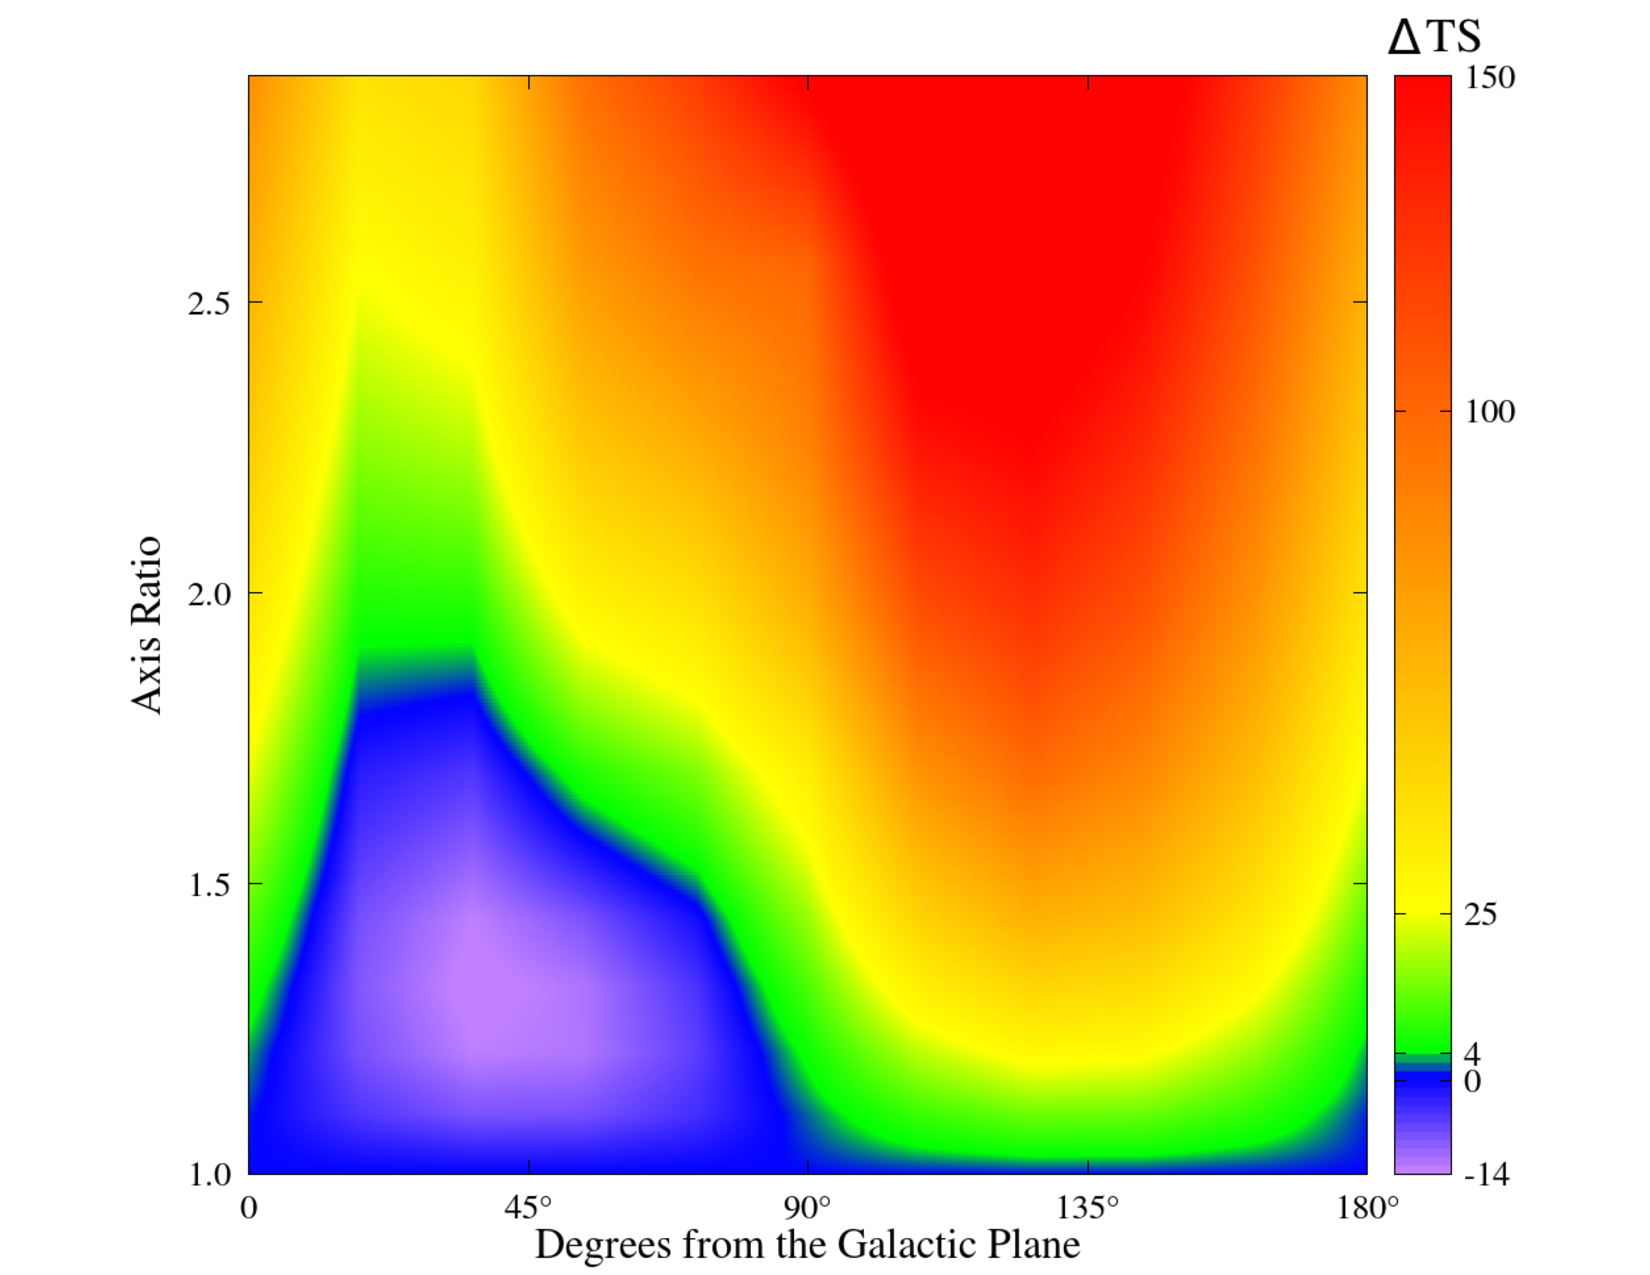
\includegraphics[width=0.48\textwidth]{figures/Daylan2014_spectra_per_channel.pdf}
	\caption{
	Prompt gamma-ray spectrum $dN_\gamma/dE_\gamma$ produced per dark matter annihilation for a 30~GeV WIMP, shown for a variety of Standard Model final states.
		Hadronic channels ($b\bar{b}$, $c\bar{c}$) produce soft, broad spectra peaked at $E_\gamma \sim m_\chi/20$, while leptonic channels ($\tau^+\tau^-$, $\mu^+\mu^-$) yield harder spectra concentrated near the kinematic endpoint.
		Figure from Daylan et al.~\cite{Daylan:2014rsa}.
	}
	\label{fig:spectra_per_channel}
\end{figure}

\subsection{Spectral Features and Signatures}
\label{sec:spectral_features}
The continuum spectra described above are broad, featureless apart from a cutoff at $m_\chi$, and not unique to dark matter --- astrophysical gamma-ray sources produce similar power-law-like spectra through conventional particle acceleration (cf.\ Section~\ref{sec:production_mechanisms}).
The discriminating power of gamma-ray searches therefore lies in spectral features that have no plausible astrophysical counterpart; and unlike charged cosmic rays, whose spectral structures are smeared by propagation through galactic magnetic fields, sharp features in the gamma-ray spectrum propagate intact from source to detector and can be searched for directly~\cite{Dermer:2009zz}.

\textbf{Monochromatic lines.}
The cleanest such feature is a gamma-ray line at $E_\gamma = m_\chi$, produced when two dark matter particles annihilate directly into a pair of photons, $\chi\chi \to \gamma\gamma$~\cite{Cirelli:2024ssz}.
Because dark matter carries no electric charge, this process cannot occur at tree level; it must proceed through quantum loops of charged particles, suppressing the cross-section by a factor of order $\alpha^2$ relative to annihilation into Standard Model final states~\cite{Bergstrom:1997fj,Cirelli:2024ssz}.
The expected flux is correspondingly small, yet no known astrophysical mechanism produces a sharp line superimposed on a smooth continuum --- the monochromatic signal has long been regarded as a ``smoking gun'' for dark matter~\cite{Bergstrom:1997fj,Bergstrom:2001jj}.
Related processes such as $\chi\chi \to \gamma Z$ or $\gamma h$ may also produce lines at lower energies, since part of the available centre-of-mass energy goes into the mass of the $Z$ or Higgs boson. 
% detecting multiple lines at predictable separations would provide a strong consistency check~\cite{Cirelli:2024ssz}.
% An exception to the generic loop suppression arises in models with non-perturbative Sommerfeld enhancement, where the line cross-section can be boosted to a level comparable with the continuum contribution for a range of dark matter masses~\cite{Cirelli:2024ssz}.

\textbf{Virtual internal bremsstrahlung (VIB).}
When a photon is radiated from a charged particle mediating the annihilation, the resulting spectrum acquires a characteristic \textit{saw-tooth} shape: rising steeply toward a sharp cutoff at $E_\gamma \lesssim m_\chi$~\cite{Bringmann:2007nk,Cirelli:2024ssz}.
In models where two-body annihilation into light fermions is suppressed, this radiative three-body channel can become the dominant process, making the saw-tooth feature the leading spectral signature~\cite{Bringmann:2007nk,Cirelli:2024ssz}.

These spectral features are illustrated schematically in Figure~\ref{fig:spectral_features}.

\begin{figure}[t]
	\centering
	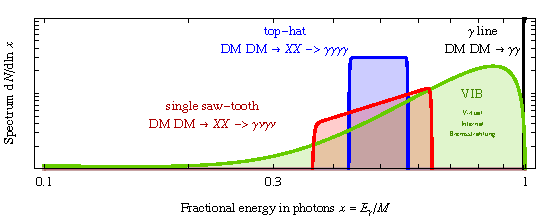
\includegraphics[width=0.85\textwidth]{figures/DMphotonSpectra.pdf}
	\caption{Notable sharp gamma-ray spectral features from dark matter annihilation, as a function of the fractional energy carried by the photon, $x = E_\gamma/m_\chi$.
		From left to right: the single saw-tooth from $\chi\chi \to XX \to \gamma\nu\gamma\nu$ (red), the ``top-hat'' (box-shaped) spectrum from cascade decays $\chi\chi \to XX \to \gamma\gamma\gamma\gamma$ (blue), the ``saw-tooth'' shape of virtual internal bremsstrahlung (VIB, green), and the monochromatic line from $\chi\chi \to \gamma\gamma$ at $E_\gamma = m_\chi$ (black).
		Unlike the case for charged cosmic rays, these sharp features propagate intact to the detector and can be searched for directly.
		Credit: Cirelli et al.~\cite{Cirelli:2024ssz}.
	}
	\label{fig:spectral_features}
\end{figure}

\textbf{Electroweak corrections.}
When the dark matter mass lies far above the electroweak scale ($m_\chi \gg M_W$), the annihilation products are energetic enough to radiate $W$ and $Z$ bosons readily --- much as a fast-moving charge emits photons --- and this radiation can no longer be neglected for heavy candidates~\cite{Ciafaloni:2010ti,Cirelli:2024ssz}.
Its effect is twofold.
First, the subsequent decays of the radiated bosons smear sharp features such as monochromatic lines and add a soft continuum of lower-energy gamma-rays.
Second, they feed final states that would otherwise be absent, so that even purely leptonic channels ($\chi\chi \to e^+e^-$, $\mu^+\mu^-$) end up producing antiprotons and every annihilation channel contributes to every messenger~\cite{Cirelli:2024ssz}.
\blue{These are corrections to the \emph{final state}, reshaping the spectrum produced per annihilation.
They should not be confused with the Sommerfeld enhancement of Section~\ref{sec:1.2.4}, which in this regime is likewise of electroweak origin: for $m_\chi \gg M_W$, the $W$ and $Z$ mediate a long-range force between the slow incoming pair~\cite{Cirelli:2024ssz}.
That effect, however, acts on the initial state and scales the annihilation rate rather than the spectrum.}

\textbf{Prompt versus secondary emission.}
The gamma-ray production mechanisms discussed so far --- pion decay, final-state radiation, lines, VIB --- all occur promptly after their parent annihilation or decay event, and are thus referred to as \textit{prompt emission} \cite{Cirelli:2024ssz,Pinetti:2021jjs}.
Prompt photons propagate freely through the Galaxy and arrive at the detector with their spectral shape intact, because the Galaxy is effectively transparent to gamma-rays below a few hundred TeV \cite{Hooper:2024}.\footnote{This transparency is specific to propagation \emph{within} the Galaxy, where pair production ($\gamma\gamma \to e^+e^-$) on the interstellar radiation field and the CMB only becomes significant at PeV energies. Over cosmological distances, by contrast, the interaction length on the extragalactic background light drops below the Hubble length already at energies $\gtrsim 100$~GeV, defining an effective gamma-ray horizon for extragalactic sources \cite{Hooper:2024}.}

Different contributions arise when the energetic electrons and positrons produced by dark matter propagate through the interstellar medium.
These leptons upscatter ambient low-energy photons to gamma-ray energies via \textit{inverse Compton scattering} (ICS; see Section~\ref{sec:leptonic}) \cite{Blumenthal:1970gc,Hooper:2024}.
The target photon field --- the interstellar radiation field (ISRF) --- consists of three components: the cosmic microwave background, optical starlight, and dust-reprocessed infrared light \cite{Strong:2007nh}.
As a representative example, a 1 TeV electron upscatters a CMB photon to $\sim 1.5$ GeV, or a UV starlight photon to $\sim 150$ GeV \cite{Cirelli:2024ssz}.
The propagating $e^\pm$ also emit \textit{bremsstrahlung} radiation when deflected by the electric fields of interstellar gas nuclei, a process that dominates their energy losses in the 1--10 GeV range near the Galactic plane where gas densities are highest \cite{Blumenthal:1970gc,Dermer:2009zz}.
These processes produce \textit{secondary} gamma-ray emission that is spatially extended and spectrally softer than the prompt component, and whose morphology depends on the magnetic field structure, gas distribution, and radiation fields of the host galaxy \cite{Strong:2007nh,Hooper:2024}.
\blue{The same $e^\pm$ population also emits \textit{synchrotron} radiation as it gyrates in the Galactic magnetic field, but for weak-scale dark matter candidates this component peaks at radio and microwave frequencies --- a 10 GeV electron in the local $\sim 5\,\mu$G field radiates near 8 GHz \cite{Cirelli:2024ssz} --- and therefore does not contribute directly to gamma-ray searches.}
Secondary emission therefore depends not only on the dark matter distribution but also on the astrophysical environment --- magnetic fields, radiation fields, gas densities --- that reprocesses the primary electrons and positrons.
Despite this additional layer of modelling uncertainty, secondary emission plays a central role in the interpretation of the Galactic Center excess discussed in Chapter~\ref{ch:4}, where the identification of the signal relies on subtracting the diffuse gamma-ray background dominated by cosmic-ray ICS and bremsstrahlung in the dense inner Galaxy \cite{Hooper:2024}.

\subsection{Dark Matter Density Profiles}
\label{sec:density_profiles}

The annihilation and decay rates \blue{presented} in Section~\ref{sec:ann_decay} depend directly on the dark matter density $\rho(r)$ --- and for annihilation, on $\rho(r)^2$.
The predicted gamma-ray flux from any astrophysical target is therefore directly related to the assumed density profile.
The same measurement constraining the particle physics simultaneously probes the dark matter distribution.

The standard profiles come from cosmological $N$-body simulations which follow the gravitational collapse of billions of dark matter particles from primordial density perturbations to the present-day cosmic web.
These simulations show that the spherically averaged density $\rho(r)$ of collapsed halos follows a logarithmic slope $s(r) \equiv d\ln\rho / d\ln r$ that steepens with radius, converging to $s \approx -3$ in the outskirts.
The behaviour in the inner region, by contrast, remains an open question --- the \textit{cusp--core problem} discussed below --- with different profiles predicting central slopes that range from a steep cusp to a constant-density core (Figure~\ref{fig:dm_profiles}).
These results can be captured by several fitting functions, each with a characteristic density $\rho_s$ and a scale radius $r_s$.

\textbf{NFW (Navarro--Frenk--White).}
The most widely adopted benchmark has a density that diverges as $\rho \propto r^{-1}$ toward the center (a ``cusp'') and falls off as $\rho \propto r^{-3}$ in the outer halo \cite{Navarro:1996gj}. It was introduced in 1997 by Navarro, Frenk, and White as a fitting function for dark matter halos in N-body simulations of cold dark matter:
%
\begin{equation}
	\rho_\text{NFW}(r) = \frac{\rho_s}{\dfrac{r}{r_s}\left(1 + \dfrac{r}{r_s}\right)^2} \,,
	\label{eq:nfw}
\end{equation}
%
A common generalization replaces the fixed inner slope with a free parameter $\gamma$, giving the ``generalized NFW'' (gNFW) profile $\rho \propto (r/r_s)^{-\gamma}(1 + r/r_s)^{\gamma - 3}$ \cite{Cirelli:2024ssz}.
The standard NFW corresponds to $\gamma = 1$; steeper values ($\gamma > 1$) describe adiabatically contracted halos, while $\gamma < 1$ accommodates shallower cusps.
This freedom is directly relevant for the Galactic Center excess analysis in Chapter~\ref{ch:4}, where the morphology of the signal constrains $\gamma$.

\textbf{Einasto.}
Originally proposed by Einasto (1965)~\cite{einasto1965construction} and later identified as a fitting function for simulated halos \cite{Cirelli:2024ssz}, this profile has a logarithmic slope that varies continuously with radius, without converging to a fixed power law at the center.
It is controlled by a shape parameter $\alpha_\text{Ein}$:

\begin{equation}
	\rho_\text{Ein}(r) = \rho_s \exp\left\{ -\frac{2}{\alpha_\text{Ein}} \left[\left(\frac{r}{r_s}\right)^{\alpha_\text{Ein}} - 1\right]\right\} \,.
	\label{eq:einasto}
\end{equation}

High-resolution simulations seem to favour Einasto over NFW as a fitting function, with $\alpha_\text{Ein} \approx 0.17$ providing a good average fit across a range of halo masses \cite{Cirelli:2024ssz}.
Nonetheless, both NFW and Einasto are commonly used as standard benchmarks.

\textbf{Burkert (cored).}
A profile with a constant-density core at small radii, it is motivated by observed rotation curves of dwarf and low-surface-brightness galaxies rather than $N$-body simulations \cite{Burkert:1995yz,Bullock:2017xww}:

\begin{equation}
	\rho_\text{Bur}(r) = \frac{\rho_s}{\left(1 + \dfrac{r}{r_s}\right)\left(1 + \left(\dfrac{r}{r_s}\right)^2\right)} \,.
	\label{eq:burkert}
\end{equation}

These three profiles are compared in Figure~\ref{fig:dm_profiles}, which shows both the radial density dependence and the fitted parameters for the Milky Way.
At large radii (around $r_\odot$) all profiles agree, but they diverge by orders of magnitude in the inner kiloparsec.

\begin{figure}[t]
	\centering
	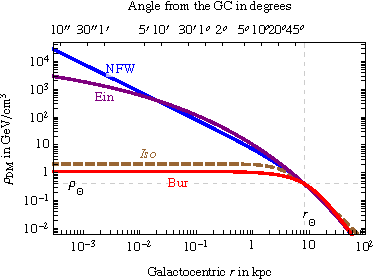
\includegraphics[width=0.75\textwidth]{figures/DMprofiles.pdf}
	\caption{Dark matter density profiles for the Milky Way: NFW (blue), Einasto (purple), Burkert (red), and Isothermal (brown) as a function of galactocentric distance.
		The profiles are normalized to agree at $r \sim r_\odot$ but diverge by orders of magnitude in the inner kiloparsec.
		Credit: Cirelli et al.~\cite{Cirelli:2024ssz}.
	}
	\label{fig:dm_profiles}
\end{figure}

When fit to the Milky Way, the parameters of these profiles are fixed by requiring consistency with the total Galactic mass ($\sim 4.7 \times 10^{11}\, M_\odot$) and the local dark matter density at the Sun's position ($r_\odot \simeq \blue{8.33}$ kpc) \cite{Cirelli:2024ssz,Pinetti:2021jjs}.
The most recent determinations place the local density at $\rho_\odot \approx 0.40 \pm 0.10$ GeV/cm$^3$ \cite{Cirelli:2024ssz}, though many analyses continue to use the historical benchmark of 0.3 GeV/cm$^3$.
Characteristic Milky Way parameters are $r_s \approx 14.5$ kpc and $\rho_s \approx 0.57$ GeV/cm$^3$ for NFW, and $r_s \approx 13.6$ kpc with $\rho_s \approx 0.15$ GeV/cm$^3$ for Einasto \cite{Cirelli:2024ssz}.

At the solar radius, all three profiles agree by construction.
They differ sharply in the inner kiloparsec, where no direct observational data constrain the dark matter profile and the resolution of current simulations reaches its limit (roughly a fraction of a kiloparsec for a Milky Way--sized halo) \cite{Cirelli:2024ssz,Navarro:1996gj,Bullock:2017xww}.
The NFW and Einasto profiles predict densities at $r \sim 100$ pc that exceed the Burkert core prediction by one to two orders of magnitude \cite{Cirelli:2024ssz}. 
% This is one of the main sources of uncertainty in indirect detection, and the choice of profile is therefore often treated as a systematic.
\blue{This is one of the main sources of uncertainty in indirect detection, and the choice of profile propagates directly into the predicted flux, as quantified in Section~\ref{sec:jfactor}.}
% This discrepancy propagates directly into the $J$-factor: the predicted gamma-ray flux from the Galactic Center can vary by orders of magnitude depending on whether one assumes a cusp or a core.

The disagreement between cuspy simulations and cored observations is known as the \textbf{cusp--core problem} \cite{Cirelli:2024ssz,Bullock:2017xww}.
Dark matter--only $N$-body simulations consistently produce cusps with inner slopes $\gamma \approx 1$--$1.5$, while rotation curve measurements --- particularly in dwarf galaxies --- often favour constant-density cores ($\gamma \approx 0$--$0.5$) \cite{Bullock:2017xww}.
Several solutions to this discrepancy have been proposed.
From the particle physics side, self-interacting dark matter \blue{(introduced in Section~\ref{sec:1.2.1})}, with $\sigma/m \approx 0.5$--$10$ cm$^2$/g, transfers heat to halo centers and produces cores of the observed size \cite{Spergel:1999mh,Tulin:2017ara,Bullock:2017xww}, while ultralight ``fuzzy'' dark matter generates solitonic cores through quantum pressure on scales comparable to the de Broglie wavelength \cite{Hu:2000ke}.
From the astrophysical side, modern hydrodynamical simulations show that repeated bursts of supernova-driven outflows can rapidly alter the central gravitational potential, pushing dark matter outward and flattening a primordial cusp into a core.
\blue{The inclusion of baryonic feedback has thus considerably relaxed the original tension --- cores of the observed size now emerge within plain $\Lambda$CDM, without invoking new dark-sector physics --- although the problem is not regarded as fully settled, since the predicted core sizes depend on phenomenological sub-grid feedback prescriptions and differ between simulation codes \cite{Cirelli:2024ssz,Bullock:2017xww}.}

The effectiveness of baryonic feedback depends non-monotonically on the stellar-to-halo mass ratio $M_\star / M_\text{vir}$: core formation peaks at intermediate ratios ($M_\star / M_\text{vir} \approx 5 \times 10^{-3}$, the regime of bright dwarfs), where supernovae are frequent enough to redistribute dark matter, but is negligible in ultrafaint dwarfs (too few stars) and in massive galaxies where adiabatic contraction recreates a cusp \cite{Cirelli:2024ssz,Bullock:2017xww}.
For the Milky Way ($M_\star / M_\text{vir} \approx 0.08$), this would place the expected inner profile in the cuspy regime, although the argument rests on the assumption that feedback and contraction have been correctly modelled, which remains a field of active research with large uncertainties.

\textbf{Substructure and boost factors.}
Real dark matter halos are not smooth.
$N$-body simulations reveal a rich hierarchy of gravitationally bound subhalos embedded within the main halo, with a mass function $dn/dM \propto M^{-2}$ extending from cluster masses down to the resolution limit \cite{Springel:2008cc,Diemand:2008in,Cirelli:2024ssz}.
Because annihilation scales as $\rho^2$, the clumpy density field produces a higher total signal than a smooth halo of the same average density.
This follows from Jensen's inequality applied to the convex function $\rho^2$: for any non-uniform density distribution, the volume-averaged squared density satisfies $\langle \rho^2 \rangle > \langle \rho \rangle^2$, with equality only for a perfectly homogeneous halo.
This enhancement is parametrized by a multiplicative boost factor $B \equiv \langle \rho^2 \rangle / \langle \rho \rangle^2$ \cite{Cirelli:2024ssz}.

Early estimates of the boost factor ranged from modest ($B \sim 10$) to extreme ($B \sim 10^9$) \cite{Bergstrom:1998jj,Calcaneo-Roldan:2000xwm,Berezinsky:2003vn,Stoehr:2003hf,Cirelli:2024ssz}, but modern analyses find much smaller values \cite{Lavalle:2007apj,Sanchez-Conde:2013yxa,Cirelli:2024ssz}.
The survival of subhalos is governed by tidal stripping from the host halo's gravitational field, gravitational ``disk shocking'' as subhalos cross the dense baryonic disk, and encounters with individual stars --- all of which preferentially destroy subhalos in the inner Galaxy \cite{Cirelli:2024ssz,Sanchez-Conde:2013yxa}.
When these effects are included, the boost factor for the Galaxy as a whole is $B \lesssim \mathcal{O}(10)$--$\mathcal{O}(30)$ \cite{Sanchez-Conde:2013yxa,Moline:2016pbm,Cirelli:2024ssz}.
Toward the Galactic Center, where subhalos are most heavily depleted by tidal forces, the boost is expected to be negligible \cite{Cirelli:2024ssz,Sanchez-Conde:2013yxa}.
The outer halo, by contrast, retains a richer subhalo population, since tidal forces weaken with galactocentric distance. These surviving subhalos --- seen preferentially at high galactic latitudes --- are the targets of the searches described in Chapter~\ref{ch:5}.

The subhalo hierarchy does not extend to arbitrarily small masses.
It is truncated at a minimum mass $M_\text{min}$ set by the kinetic decoupling of the dark matter particle from the thermal plasma in the early universe \cite{Cirelli:2024ssz}.
After kinetic decoupling, dark matter particles free-stream over a characteristic length $\lambda_\text{fs}$, erasing density perturbations below the corresponding mass scale $M_\text{min} \simeq (4\pi/3)\, \rho_\text{DM}\, \lambda_\text{fs}^3$ \cite{Cirelli:2024ssz}.
For a 100 GeV WIMP with weak-scale couplings, $M_\text{min} \sim 10^{-6}\, M_\odot$ --- roughly an Earth mass \cite{Cirelli:2024ssz}.
This scale lies far below the resolution of any current simulation and represents a fundamental uncertainty in the predicted total annihilation rate, since the integral over the subhalo mass function is dominated by the smallest masses.

The density profiles and substructure properties introduced here feed directly into the $J$-factor and $D$-factor formalism of Section~\ref{sec:jfactor}.

\subsection{The Flux Factorization: $J$-Factor and $D$-Factor}
\label{sec:jfactor}

Combining the particle physics of Section~\ref{sec:ann_decay} with the density profiles of Section~\ref{sec:density_profiles}, we can now write the differential gamma-ray flux from dark matter annihilation observed from a direction $\psi$ relative to the Galactic Center \cite{Cirelli:2024ssz,Hooper:2024}:

\begin{equation}
	\frac{d\Phi_\gamma}{dE\, d\Omega} = \underbrace{\frac{1}{4\pi} \frac{\langle \sigma v_\text{rel} \rangle}{2 m_\chi^2} \frac{dN_\gamma}{dE}}_{\text{Particle Physics}} \quad \times \underbrace{J(\psi)}_{\text{Astrophysics}} \,.
	\label{eq:flux_ann}
\end{equation}

The prefactor $1/(4\pi)$ reflects the isotropic emission of photons over the full sphere, and the factor of $1/2$ avoids double-counting for self-conjugate (Majorana) particles, as discussed in Section~\ref{sec:ann_decay}.
The $J$-factor is the line-of-sight integral of the density squared:
%
\begin{equation}
	J(\psi) = \int_\text{l.o.s.} \rho^2\bigl(r(s, \psi)\bigr) \, ds \,,
	\label{eq:jfactor}
\end{equation}
%
where $s$ parametrizes the distance along the line of sight and $r$ is the galactocentric radius, related to $s$ and the observation angle $\psi$ by $r = (r_\odot^2 + s^2 - 2 r_\odot s \cos\psi)^{1/2}$, with $r_\odot \simeq 8.33$ kpc the Sun--Galactic Center distance \cite{Cirelli:2024ssz}.
In this dimensionful convention, $J$ carries units of GeV$^2$ cm$^{-5}$.
An alternative dimensionless definition, in which $\rho$ and $s$ are normalized to $\rho_\odot$ and $r_\odot$ respectively, is also often used in the literature \cite{Cirelli:2024ssz}.

For decaying dark matter, the analogous expression is \cite{Cirelli:2024ssz,Pinetti:2021jjs}:

\begin{equation}
	\frac{d\Phi_\gamma}{dE\, d\Omega} = \frac{1}{4\pi} \frac{\Gamma}{m_\chi} \frac{dN_\gamma}{dE} \times D(\psi) \,,
	\label{eq:flux_dec}
\end{equation}

where $\Gamma = 1/\tau$ is the decay rate.
No symmetry factor appears, since decay is a single-particle process.
The $D$-factor is:
%
\begin{equation}
	D(\psi) = \int_\text{l.o.s.} \rho\bigl(r(s, \psi)\bigr) \, ds \,,
	\label{eq:dfactor}
\end{equation}
%
and carries units of GeV cm$^{-2}$.
Because $D$ depends on $\rho$ rather than $\rho^2$, it is far less sensitive to the assumed density profile than the $J$-factor, making decay searches less model-dependent than their annihilation counterparts.
Beyond this technical difference, the two processes are interesting for different reasons.
Annihilation is the characteristic signature of thermal-relic WIMPs, whose present-day cross-section is tied to the observed relic abundance (Section~\ref{sec:1.2}) \cite{Bertone:2004pz}, and the $\rho^2$ weighting makes the densest concentrations of dark matter --- the Galactic Center and individual subhalos --- the most rewarding targets.
Decay, by contrast, is the natural channel for feebly-coupled or non-thermal candidates such as sterile neutrinos \cite{Dodelson:1993je,Boyarsky:2018tvu} and axion-like particles \cite{Arias:2012az}, whose only requirement is a lifetime exceeding the age of the universe; the linear $\rho$ weighting instead favours large, diffuse targets that maximise the enclosed mass --- the outer Galactic halo, galaxy clusters, the isotropic background \cite{Ibarra:2013cra}, and even cosmic-web filaments, where an annihilation signal would be suppressed \cite{Pinetti:2021jjs,Cirelli:2024ssz}.

The particle physics factor --- containing $m_\chi$, $\langle \sigma v_\text{rel} \rangle$ (or $\tau$), and the spectral shape $dN_\gamma/dE$ --- encodes the dark matter model we wish to test.
The astrophysical factor --- $J$ or $D$ --- encodes the distribution of dark matter along the line of sight, determined by the density profile of the host halo and constrained independently through kinematic measurements.
A non-detection translates directly into an upper limit on $\langle \sigma v_\text{rel} \rangle$ for annihilation; and an upper limit on $\Gamma$ (equivalently, a lower limit on $\tau$) for decay.

When applied to an extended region of the sky, the integrated flux is obtained by integrating $J$ (or $D$) over the solid angle of interest.
For comparing different targets, one typically quotes the $J$-factor integrated over a cone of half-angle $\theta_\star$ centered on the target:

\begin{equation}
	J_\text{int}(\theta_\star) = \int_0^{\theta_\star} J(\psi) \, 2\pi \sin\psi \, d\psi \,.
	\label{eq:jfactor_int}
\end{equation}

For dwarf spheroidal galaxies observed by Fermi-LAT, typical integrated $J$-factors (within $\theta_\star = 0.5^\circ$) range from $\sim 10^{16}$ to $\sim 10^{19.5}$ GeV$^2$ cm$^{-5}$, depending on the system's mass, distance, and the quality of the kinematic data used to reconstruct its density profile \cite{Hooper:2024,Cirelli:2024ssz,Bonnivard:2015xpq}.
The choice of integration angle reflects the angular extent of the target: dSphs are resolved by Fermi-LAT and extended emission can be recovered within $\sim 0.5^\circ$, while dark matter subhalos at typical Galactic distances are unresolved and effectively point-like, so their $J$-factors are integrated within $\theta_\star \sim 0.1^\circ$, matching the instrument's point-spread function.
% These values are orders of magnitude smaller than the Galactic Center $J$-factor, but the absence of astrophysical backgrounds in dwarfs compensates for the reduced signal.
\blue{These values are orders of magnitude smaller than the Galactic Center $J$-factor (cf.\ the signal-versus-background comparison in Section~\ref{sec:targets}).}

Several caveats affect the simple factorization above.
First, it assumes a \textit{velocity-independent} annihilation cross-section.
If $\langle \sigma v_\text{rel} \rangle$ depends on the dark matter velocity --- as it does for $p$-wave annihilation ($\sigma v \propto v^2$) or Sommerfeld-enhanced models ($\sigma v \propto 1/v$) --- the cross-section can no longer be factored out of the line-of-sight integral \cite{Cirelli:2024ssz}.
In such cases, one must compute an \textit{effective $J$-factor} that folds the full, position-dependent velocity distribution into the integral, and the clean particle-physics/astrophysics separation is lost.

Second, even for velocity-independent cross-sections, the $J$-factor depends quadratically on the density profile, making it extremely sensitive to the uncertainties discussed in Section~\ref{sec:density_profiles}.
For the Galactic Center, the $J$-factor computed with an NFW profile can exceed the Burkert value by orders of magnitude \cite{Cirelli:2024ssz}; even within the NFW paradigm, varying the inner slope from $\gamma = 0.7$ to $\gamma = 1.3$ changes the predicted flux by more than an order of magnitude \cite{Hooper:2024}.
The astrophysical factor is therefore the dominant systematic uncertainty in annihilation searches \blue{for a given dark matter model}.

\subsection{Observational Targets for Gamma-Ray Searches}
\label{sec:targets}

To maximise the gamma-ray signal from dark matter, one should observe targets with large $J$-factors (for annihilation) or $D$-factors (for decay) and low astrophysical backgrounds.
No single target satisfies both criteria simultaneously, and the field has consequently developed a multi-target observation programme in which the complementary strengths of different targets compensate each other's weaknesses.
We now review the principal targets, noting their advantages, limitations, and connection to the analyses developed in this thesis.

\textbf{The Galactic Center.}
The center of the Milky Way offers the largest $J$-factor of any astronomical source, owing to its proximity ($\sim 8$ kpc) and the expected steep rise of the dark matter density at small radii \cite{Hooper:2024}. \blue{In the inner $40^\circ \times 40^\circ$ region, the physical $J$-factor is approximately $J \sim 10^{23}~\mathrm{GeV}^2\,\mathrm{cm}^{-5}\,\mathrm{sr}$ \cite{Chang_2018}.}
For an NFW profile with $\gamma = 1$ and a local density $\rho_\odot = 0.4$ GeV/cm$^3$, the predicted flux from the inner $10^\circ$ exceeds that from any individual dwarf galaxy by more than three orders of magnitude \cite{Hooper:2024}.
If a steeper inner slope ($\gamma \approx 1.3$) is assumed, the flux increases by an additional factor of $\sim 5$; for a shallower slope ($\gamma \approx 0.7$) it decreases by $\sim 3$ \cite{Hooper:2024}.
In either case, the Galactic Center remains the brightest expected source of dark matter annihilation products on the sky.

The advantage is offset by severe astrophysical contamination.
The inner few degrees of the Galaxy feature a bright diffuse emission from cosmic-ray protons and electrons scattering off interstellar gas (through pion production and bremsstrahlung) and ambient radiation fields (through inverse Compton scattering), together with numerous point sources --- supernova remnants, pulsars, and the central supermassive black hole \cite{Hooper:2024}.
Models of this diffuse foreground (see Section~\ref{sec:gde_model}) are constructed from gas maps and the locally measured cosmic-ray spectrum, and while they capture the broad features of the observed emission, they cannot account for its detailed spectral and morphological structure.
This imperfect background knowledge is the primary obstacle to extracting a dark matter signal from the Galactic Center.

Despite these difficulties, the Fermi-LAT has detected a statistically significant excess of gamma-rays from the inner Galaxy at energies between $\sim 0.5$ and 5 GeV --- the so-called Galactic Center excess (GCE) \cite{Goodenough:2009gk,Hooper:2010mq,Daylan:2014rsa}.
The spectrum and approximately spherical morphology of this excess are consistent with the predictions for a $\sim \blue{35}$--$\blue{50}$ GeV dark matter particle annihilating into $b\bar{b}$ quarks at a rate close to the thermal relic value \cite{Daylan:2014rsa}.
The dark matter interpretation is compelling, but an unresolved population of millisecond pulsars in the Galactic bulge provides an equally plausible astrophysical explanation.
Multiple statistical analyses have investigated the point-source versus diffuse origin of the excess, reaching contradictory conclusions.
The morphological debate --- whether the excess traces a spherical dark matter halo or the stellar distribution of the Galactic bulge --- remains unresolved.
This persistent ambiguity motivates the dedicated analysis in Chapter~\ref{ch:4}, which examines the millisecond pulsar hypothesis by constraining the pulsar luminosity function from globular cluster observations.

\textbf{Dwarf spheroidal galaxies.}
The Milky Way's satellite dwarf galaxies occupy the opposite end of the signal-versus-background trade-off.
% Dwarf spheroidals are among the most dark matter--dominated objects known: their shallow gravitational potential wells allowed early supernova feedback to expel most of the baryonic gas, halting star formation and leaving behind systems with mass-to-light ratios ranging from tens of $M_\odot/L_\odot$ for classical dwarfs like Sculptor to thousands for ultrafaint dwarfs such as Segue~1 \cite{Cirelli:2024ssz}.
\blue{Dwarf spheroidals are among the most dark matter--dominated objects known (Section~\ref{sec:1.1.1}): their shallow gravitational potential wells allowed early supernova feedback to expel most of the baryonic gas, halting star formation and leaving behind systems with extreme mass-to-light ratios.}
The scarcity of stars, gas, and other active astrophysical objects means that their gamma-ray backgrounds are subdominant \cite{Cirelli:2024ssz}.
% The expected dark matter flux from any individual dwarf is far smaller than from the Galactic Center --- roughly three orders of magnitude lower for a typical system \cite{Hooper:2024} --- but the absence of competing emission makes them the cleanest targets available.
\blue{The expected dark matter flux from any individual dwarf is far smaller than from the Galactic Center, as quantified above, but the absence of competing emission makes them the cleanest targets available.}

Eight ``classical'' dwarf spheroidals (Sculptor, Fornax, Leo I and II, Ursa Minor, Draco, Carina, and Sextans) have been known since before the 1990s \cite{Cirelli:2024ssz}.
The advent of digital surveys --- SDSS, DES, and Gaia --- has brought the total to about fifty confirmed ultrafaint dwarfs, with roughly ten more candidates awaiting spectroscopic confirmation \cite{Pace:2024sys}.
This growing census is expected to continue with the Rubin Observatory.

By combining observations of dozens of these systems in a stacked analysis, the Fermi-LAT collaboration has derived some of the tightest constraints on the annihilation cross-section to date \cite{Fermi-LAT:2015att,2024PhRvD.109f3024M,Hooper:2024}.
% The original combined analysis of 15 kinematically confirmed dSphs excluded the thermal relic cross-section ($\langle \sigma v_\text{rel} \rangle \simeq 2.2 \times 10^{-26}$ cm$^3$/s) for dark matter masses below $\sim 100$ GeV in the $b\bar{b}$ channel \cite{Fermi-LAT:2015att}; the most recent legacy analysis extends this to 50 dSphs with 14 years of data, yielding slightly tighter constraints in the 20--100 GeV mass range while confirming the earlier exclusion \cite{2024PhRvD.109f3024M}.
\blue{These stacked analyses exclude the thermal relic cross-section for dark matter masses below $\sim 100$ GeV in the $b\bar{b}$ channel; the current numbers, and their evolution from 15 to 50 dwarfs, are collected in Section~\ref{sec:status} \cite{Fermi-LAT:2015att,2024PhRvD.109f3024M}.}
The dominant systematic uncertainty lies in the $J$-factors themselves, which must be inferred from the kinematics of the dwarfs' constituent stars.
For ultrafaint systems, the number of kinematic tracers can be extremely small, and removing or adding a single star from the sample can shift the reconstructed $J$-factor by orders of magnitude \cite{Cirelli:2024ssz}.
Additional systematics arise from the cusp--core ambiguity in the inner density profile and from the choice of integration angle $\theta_\star$ \cite{Cirelli:2024ssz}.
Despite these challenges, dwarfs remain the gold standard for model-independent constraints.
Chapter~\ref{ch:5} of this thesis searches for dark matter subhalos --- which may include unassociated dwarf satellites --- among the unidentified Fermi-LAT sources.
%, while Chapter~\ref{ch:6} develops methods to characterize the unresolved gamma-ray source population as a whole.

\textbf{Dark subhalos.} $\Lambda$CDM simulations predict far more gravitationally bound subhalos within the Milky Way's halo than the $\sim 50$ known satellite galaxies can account for \cite{Springel:2008cc,Bullock:2017xww}.
Most of these subhalos are expected to be entirely dark --- devoid of stars and gas --- yet \blue{some of them may be sufficiently massive} to produce a detectable gamma-ray flux if the annihilation cross-section is near the thermal relic value.
Such dark subhalos would appear in the Fermi-LAT data as unassociated point sources with no counterpart at other wavelengths.
Their positions are unknown a priori, turning the search into a classification problem: distinguishing rare dark matter subhalos from the much larger population of unidentified astrophysical sources (primarily pulsars and faint blazars).
This challenge is addressed in Chapter~\ref{ch:5}, where machine learning methods are applied to \blue{search for} unassociated Fermi-LAT sources in the presence of dataset shift between simulations and real data.

\textbf{The unresolved gamma-ray background.}
The cumulative, nearly isotropic gamma-ray flux that remains after subtracting resolved point sources and Galactic diffuse emission constitutes the unresolved gamma-ray background (UGRB) \cite{DGRB-review}.
Chapters~\ref{ch:6} and~\ref{ch:7} develop methods to characterize the unresolved source populations that compose the UGRB.
This unresolved background receives contributions from unresolved blazars (BL~Lac objects and flat-spectrum radio quasars), misaligned active galactic nuclei, star-forming galaxies, and millisecond pulsars (see Section~\ref{sec:astro_sky}) \cite{DGRB-review}.
Unresolved BL~Lac objects alone can account for the majority of the UGRB above $\sim 100$ GeV, while at lower energies other populations are required \cite{DGRB-review}.
A dark matter component --- originating from annihilation or decay in all halos and subhalos across cosmic history --- may also be present, but it is expected to be subdominant in the total intensity spectrum \cite{DGRB-review,Cirelli:2024ssz}.

Because the dark matter signal is potentially hidden beneath dominant astrophysical foregrounds, its extraction requires methods that go beyond the energy spectrum alone.
The angular anisotropies of the UGRB carry additional information: different source classes imprint different patterns of spatial fluctuations, reflecting their distinct clustering properties, redshift distributions, and luminosity functions.
Cross-correlating these anisotropies with independent gravitational tracers of the large-scale structure --- galaxy catalogs, cosmic shear from weak lensing surveys, or $21\,$cm intensity mapping of neutral hydrogen --- can isolate the component that traces the dark matter distribution \cite{DGRB-review,Pinetti:2021jjs,Cirelli:2024ssz}.
The approach is particularly powerful because dark matter annihilation scales as $\rho^2$ and has a redshift evolution distinct from that of astrophysical gamma-ray emitters, providing a spectral and tomographic handle for separation.
This cross-correlation technique forms the basis of the analysis in Chapter~\ref{ch:8}, where the sensitivity of next-generation instruments to the dark matter cross-correlation signal is forecast.

The complementary strengths of these targets motivate the multi-target programme developed in Parts II through IV of this thesis.
Each target exposes different aspects of the dark matter parameter space and is sensitive to different systematic uncertainties.

\subsection{Multi-Messenger Context}
\label{sec:multi_messenger}

\blue{We argued that, if dark matter annihilates or decays, it could produce stable Standard Model particles, not only gamma-rays.
Each messenger would open a complementary window onto the dark sector, with its own advantages and limitations.}

\textbf{Neutrinos} share the key advantage of photons --- having no electrical charge --- and therefore propagate in straight lines, preserving directional information \cite{Cirelli:2024ssz,Hooper:2024}.
They can also escape environments opaque to photons: dark matter captured in the solar core, for instance, annihilates into neutrinos that are the only annihilation products to reach the surface, making high-energy solar neutrinos a probe of the dark matter--nucleon scattering cross-section \cite{Cirelli:2024ssz}.
Searches by IceCube, ANTARES, and Super-Kamiokande have found no signal, but for dark matter masses below a few hundred GeV they set bounds on the spin-dependent cross-section roughly one order of magnitude stronger than direct detection experiments \cite{IceCube:2016dgk,Cirelli:2024ssz}.
For galactic targets, however, neutrino constraints remain generally weaker than the corresponding gamma-ray bounds, becoming competitive only above roughly 1--10 TeV depending on the annihilation channel \cite{Cirelli:2024ssz}.

\textbf{Charged cosmic rays} --- electrons, positrons, antiprotons, and heavier anti-nuclei --- suffer from a fundamental limitation: galactic magnetic fields randomize their arrival directions, erasing all spatial information and leaving only the energy spectrum as the main observable \cite{Cirelli:2024ssz,Pinetti:2021jjs}.
The positron fraction measured by PAMELA and AMS-02 rises steeply above 10 GeV \cite{PAMELA:2008gwm,Cirelli:2024ssz}, but fitting it with dark matter requires a cross-section three orders of magnitude above the thermal relic value, in severe tension with gamma-ray and CMB constraints; the excess is now widely attributed to nearby pulsars \cite{Cirelli:2024ssz,Hooper:2024}.
AMS-02 antiproton data show a tentative excess at 10--20 GeV compatible with an $\sim$80 GeV dark matter particle annihilating into $b\bar{b}$ at roughly the thermal cross-section \cite{Cuoco:2016eej,Cirelli:2024ssz}.
These parameters overlap with those invoked for the Galactic Center excess (Chapter~\ref{ch:4}), but the significance drops below $\sim 2\sigma$ once systematic uncertainties in the propagation model and production cross-sections are included \cite{Cirelli:2024ssz}.
Low-energy anti-deuterons and anti-helium have generally low astrophysical backgrounds, so their detection would be a qualitatively different signature.
AMS-02 and the upcoming GAPS experiment may reach the sensitivity needed to probe the thermal relic cross-section \cite{Cirelli:2024ssz,Hooper:2024}.

\textbf{CMB} --- \blue{An independent and increasingly powerful constraint comes from the \CMB, whose physics we introduced in Section~\ref{sec:1.3}: dark matter annihilation during and after recombination injects energy into the photon--baryon plasma, distorting the temperature and polarisation anisotropies in a way that is tightly bounded by Planck data \cite{Aghanim:2018eyx}.
For $s$-wave annihilation, these bounds exclude the thermal relic cross-section below roughly $30$~GeV in leptonic channels and $10$--$15$~GeV in hadronic ones \cite{Aghanim:2018eyx,Hooper:2024} --- limits that are largely independent of astrophysical modelling and therefore highly complementary to gamma-ray searches.}

% This thesis focuses exclusively on \textbf{gamma-rays} --- the messenger that provides both spatial and spectral information while relying on the fewest assumptions about particle propagation.
% Multi-messenger results are noted where they bear on the gamma-ray analyses, but the searches in Parts II--V rely entirely on the gamma-ray formalism developed above.

\subsection{The Status of the Field}
\label{sec:status}

\blue{Despite decades} of increasingly sensitive searches across all three detection strategies, no unambiguous signal of dark matter has been found.
The current status is best summarized as a set of progressively tightening bounds on the cross-section and decay lifetime, with a few anomalies whose dark matter interpretations have been challenged by plausible astrophysical alternatives.

\textbf{Gamma-ray constraints.}
The tightest indirect detection limits come from the Fermi-LAT stacked analysis of Milky Way dwarf spheroidal galaxies.
The original combined analysis of 15 dSphs with six years of data excluded the thermal relic cross-section for dark matter masses in the range $\sim 10$--$100$ GeV in the $b\bar{b}$ channel \cite{Fermi-LAT:2015att}; below $\sim 10$ GeV the Fermi-LAT effective area drops steeply and the constraints weaken.
The most recent legacy analysis extends the sample to 50 dSphs and 14 years of Fermi-LAT exposure, confirming and slightly strengthening these constraints \cite{2024PhRvD.109f3024M,Hooper:2024}; no significant excess is found in the combined likelihood analysis, though a marginal ($2$--$3\sigma$ local) excess near $M_\chi \approx 150$--$230$ GeV in the $b\bar{b}$ channel has motivated projections for future observations \cite{2024PhRvD.109f3024M}.
For a generic annihilation channel, marginalizing over branching ratios yields a model-independent lower limit of $m_\chi \gtrsim 20$ GeV \cite{Cirelli:2024ssz}.
Constraints on the dark matter lifetime, derived primarily from the isotropic gamma-ray background and Milky Way halo observations, reach $\tau \gtrsim 10^{27}$--$10^{28}$ seconds depending on the decay channel and dark matter mass --- about ten orders of magnitude longer than the age of the universe \cite{Cohen:2016uyg,Blanco_2019,Cirelli:2024ssz}.

\textbf{Direct detection and collider constraints.}
% The tightening of parameter space is not confined to indirect searches.
The current generation of dual-phase liquid xenon detectors --- LZ, XENONnT, and PandaX-4T --- has pushed the spin-independent WIMP--nucleon cross-section below $10^{-46}$ cm$^2$ for masses near the electroweak scale \blue{(see Section~\ref{sec:1.3} for the experiments and bounds)} \cite{Cirelli:2024ssz,Hooper:2024}.
At the LHC, mono-jet and mono-photon searches have found no evidence for new physics, excluding strongly interacting superpartners (squarks, gluinos) up to masses of 1--2 TeV and charged superpartners up to several hundred GeV \cite{Cirelli:2024ssz,Hooper:2024}.
% The theoretical basis of the most popular WIMP candidate --- the supersymmetric neutralino --- has been substantially weakened by the absence of supersymmetry at collider energies \cite{Cirelli:2024ssz}.

\textbf{Unresolved anomalies.}
Several persistent anomalies keep the possibility of discovery alive.
% The Galactic Center gamma-ray excess --- a signal first reported in 2009 and consistent with a $\sim$40--70 GeV dark matter particle annihilating into $b\bar{b}$ at the thermal cross-section --- remains the most debated \cite{Daylan:2014rsa,Cirelli:2024ssz,Hooper:2024}.
\blue{The Galactic Center excess, first reported in 2009, remains the most debated (its spectrum and morphology are described in Section~\ref{sec:targets}) \cite{Daylan:2014rsa,Cirelli:2024ssz,Hooper:2024}.}
% Its leading astrophysical competitor, an unresolved population of millisecond pulsars in the Galactic bulge, has been alternately supported and challenged by photon-count statistics, morphological analyses, and luminosity function arguments \cite{Cirelli:2024ssz}.
Chapter~\ref{ch:4} of this thesis contributes directly to this debate by challenging the leading astrophysical interpretation of the excess as an unresolved population of millisecond pulsars, further highlighting the complexity of the issue.
Other excesses, by contrast, admit a more satisfying astrophysical explanation.
The charged cosmic-ray anomalies discussed in Section~\ref{sec:multi_messenger} --- the AMS-02 antiproton signal and the rise in the positron fraction --- remain consistent with conventional astrophysical sources once systematic uncertainties are fully accounted for \cite{Cirelli:2024ssz,Hooper:2024}.
\blue{A similar pattern extends beyond gamma-rays: the 511~keV positron-annihilation line from the Galactic bulge admits light dark-matter interpretations alongside plausible astrophysical ones; the 3.5~keV X-ray line, once attributed to sterile-neutrino decay, is now disfavoured; and the DAMA/LIBRA annual modulation remains unconfirmed by experiments with the same NaI target \cite{Cirelli:2024ssz}.}

\blue{\textbf{Small-scale structure tensions.}
A different class of problem concerns the small-scale predictions of $\Lambda$CDM itself.
Alongside the cusp--core problem of Section~\ref{sec:density_profiles} and the ``missing satellites'' deficit --- now largely resolved by the low galaxy-formation efficiency of small halos and the discovery of ultrafaint dwarfs --- several tensions catalogued by Bullock and Boylan-Kolchin remain open: the most massive simulated subhalos appear too centrally dense to host any observed satellite (\textit{too-big-to-fail}); dwarfs of similar maximum circular velocity display remarkably different inner profiles (the \textit{diversity of rotation curves}); and the satellites of the Milky Way and Andromeda align in thin, apparently corotating planes that simulations struggle to reproduce.
These tensions motivate self-interacting (Section~\ref{sec:1.2.1}) and warm dark matter, but remain entangled with baryonic feedback modelling: for now they constrain the nature of dark matter rather than reveal it \cite{Bullock:2017xww}.}

\textbf{The methodological case for this thesis.}
Taken together, these results define the landscape in which this thesis is situated.
The viable parameter space for the simplest thermal WIMP models has narrowed substantially --- what Cirelli et al.
describe as a field ``at a turning point'' \cite{Cirelli:2024ssz}.
The standard approach to indirect detection --- searching for a bright, spectrally distinctive excess from a single target above the astrophysical background --- has not yet delivered an unambiguous discovery.
Nonetheless, the thermal relic benchmark is not the prediction of a specific model but a cosmological target: if dark matter is a thermal relic, the annihilation cross-section must have the value that produces the observed abundance, regardless of the underlying theory.
Current exclusions cover only a portion of the mass range and a subset of annihilation channels; heavier candidates, leptonic final states, and velocity-dependent cross-sections remain largely unexplored.
Extracting these signals demands methods that go beyond simple signal-over-background thresholding.

% The analyses of this thesis pursue that transition.
The Galactic Center excess demands careful modelling of the interstellar emission and the unresolved point-source population --- distinguishing dark matter annihilation from millisecond pulsars requires statistical tools, not a single spectral fit (Chapter~\ref{ch:4}).
Individual dark matter subhalos among the Fermi-LAT unassociated sources cannot be identified by classification alone; a fully probabilistic model that accounts for both covariate and prior probability shifts between associated and unassociated sources is needed to derive statistically rigorous constraints (Chapter~\ref{ch:5}).
Below the point-source detection threshold, deep learning applied to gamma-ray sky maps can recover the source-count distribution of faint populations down to fluxes a factor of 50 below the Fermi-LAT sensitivity limit, while probabilistic catalogues extend spatial source information into the sub-threshold regime (Chapters~\ref{ch:6} and \ref{ch:7}).
Finally, at the largest scales, the dark matter contribution to the unresolved gamma-ray background can potentially be isolated through its cross-correlation with independent tracers of the large-scale structure (Chapter~\ref{ch:8}).

% The mathematical framework developed in this section --- the flux factorization, the $J$-factor and $D$-factor formalism, the density profiles and their uncertainties --- underpins every one of these analyses.

